\section{DocViRe Benchmark}
\label{sec:dataset}

Existing visual document retrieval benchmarks such as ViDoRe are defined at the \emph{page} level: queries typically target local evidence within a single page, and systems are evaluated by whether they retrieve the correct page. In contrast, the task studied here takes the whole document as the retrieval unit, where relevance depends on document-level topic, cross-page information, and global semantics. Page-level annotations in ViDoRe therefore cannot be directly reused as document-level ground truth. Moreover, existing benchmarks are not designed for the cross-document document-ranking setting considered in this work. We thus construct \textbf{DocViRe}, a benchmark explicitly designed for \emph{document-level} visual retrieval.

DocViRe is designed to support document-level retrieval with document-grounded queries and multi-positive relevance annotations, while covering cross-document retrieval across multiple domains and providing a reference training set for fine-tuning trainable retrievers.

Documents are collected from the public PDFA dataset \citep{pdfa_hf_2024}. We consider seven domains: biology, education, finance, government, industrial, legal, and research.

\begin{sloppypar}
Table~\ref{tab:dataset} reports the train and test split per domain, including query and document counts. In total, the training set contains 10,884 queries and 4,438 documents. The test set contains 2,237 queries and 3,850 documents. The training and test splits are constructed from two disjoint document pools with no document overlap, ensuring that evaluation is performed on unseen documents rather than re-queried instances from the training corpus. These splits are designed to support both fine-tuning of trainable retrievers and standardized evaluation for document-level retrieval. Queries and ground-truth document sets are obtained through the construction pipeline described below. Figure~\ref{fig:dataset-pipeline} summarizes that pipeline. We describe the four steps in the following paragraphs.
\end{sloppypar}
\medskip
\begin{table*}[t]
\centering
\footnotesize
\caption{DocViRe benchmark statistics per domain (training set and test set). The train and test splits are document-disjoint. All in English.}
\label{tab:dataset}
\renewcommand{\arraystretch}{1.05}
\setlength{\tabcolsep}{0.8em}
\begin{tabular*}{\linewidth}{@{}l@{\extracolsep{\fill}}r@{\hspace{1.5em}}r@{\hspace{2.5em}}r@{\hspace{1.5em}}r@{\hspace{2em}}>{\raggedright\arraybackslash}p{0.45\linewidth}@{}}
\toprule
\multirow{2}{*}{\textbf{Domain}} & \multicolumn{2}{c}{\textbf{Training}} & \multicolumn{2}{c}{\textbf{Test}} & \multirow{2}{*}{\textbf{Description}} \\
\cmidrule(lr){2-3} \cmidrule(lr){4-5}
& \textbf{Queries} & \textbf{Docs} & \textbf{Queries} & \textbf{Docs} & \\
\midrule
Biology    & 427  & 310 & 101 & 550 & Life sciences and biology textbooks and materials \\
Education  & 2,424 & 956 & 975 & 550 & Educational and pedagogical content and resources \\
Finance    & 2,490 & 689 & 315 & 550 & Financial reports, analysis, and market data \\
Government & 1,002 & 654 & 242 & 550 & Administrative, policy, and regulatory documents \\
Industrial & 2,198 & 773 & 136 & 550 & Industrial and manufacturing processes and standards \\
Legal      & 911  & 431 & 207 & 550 & Legal and regulatory compliance and contracts \\
Research   & 1,432 & 625 & 261 & 550 & Scientific and academic research publications and papers \\
\midrule
\textbf{Total} & \textbf{10,884} & \textbf{4,438} & \textbf{2,237} & \textbf{3,850} & \\
\bottomrule
\end{tabular*}
\end{table*}
\medskip

\begin{figure}[H]
  \centering
  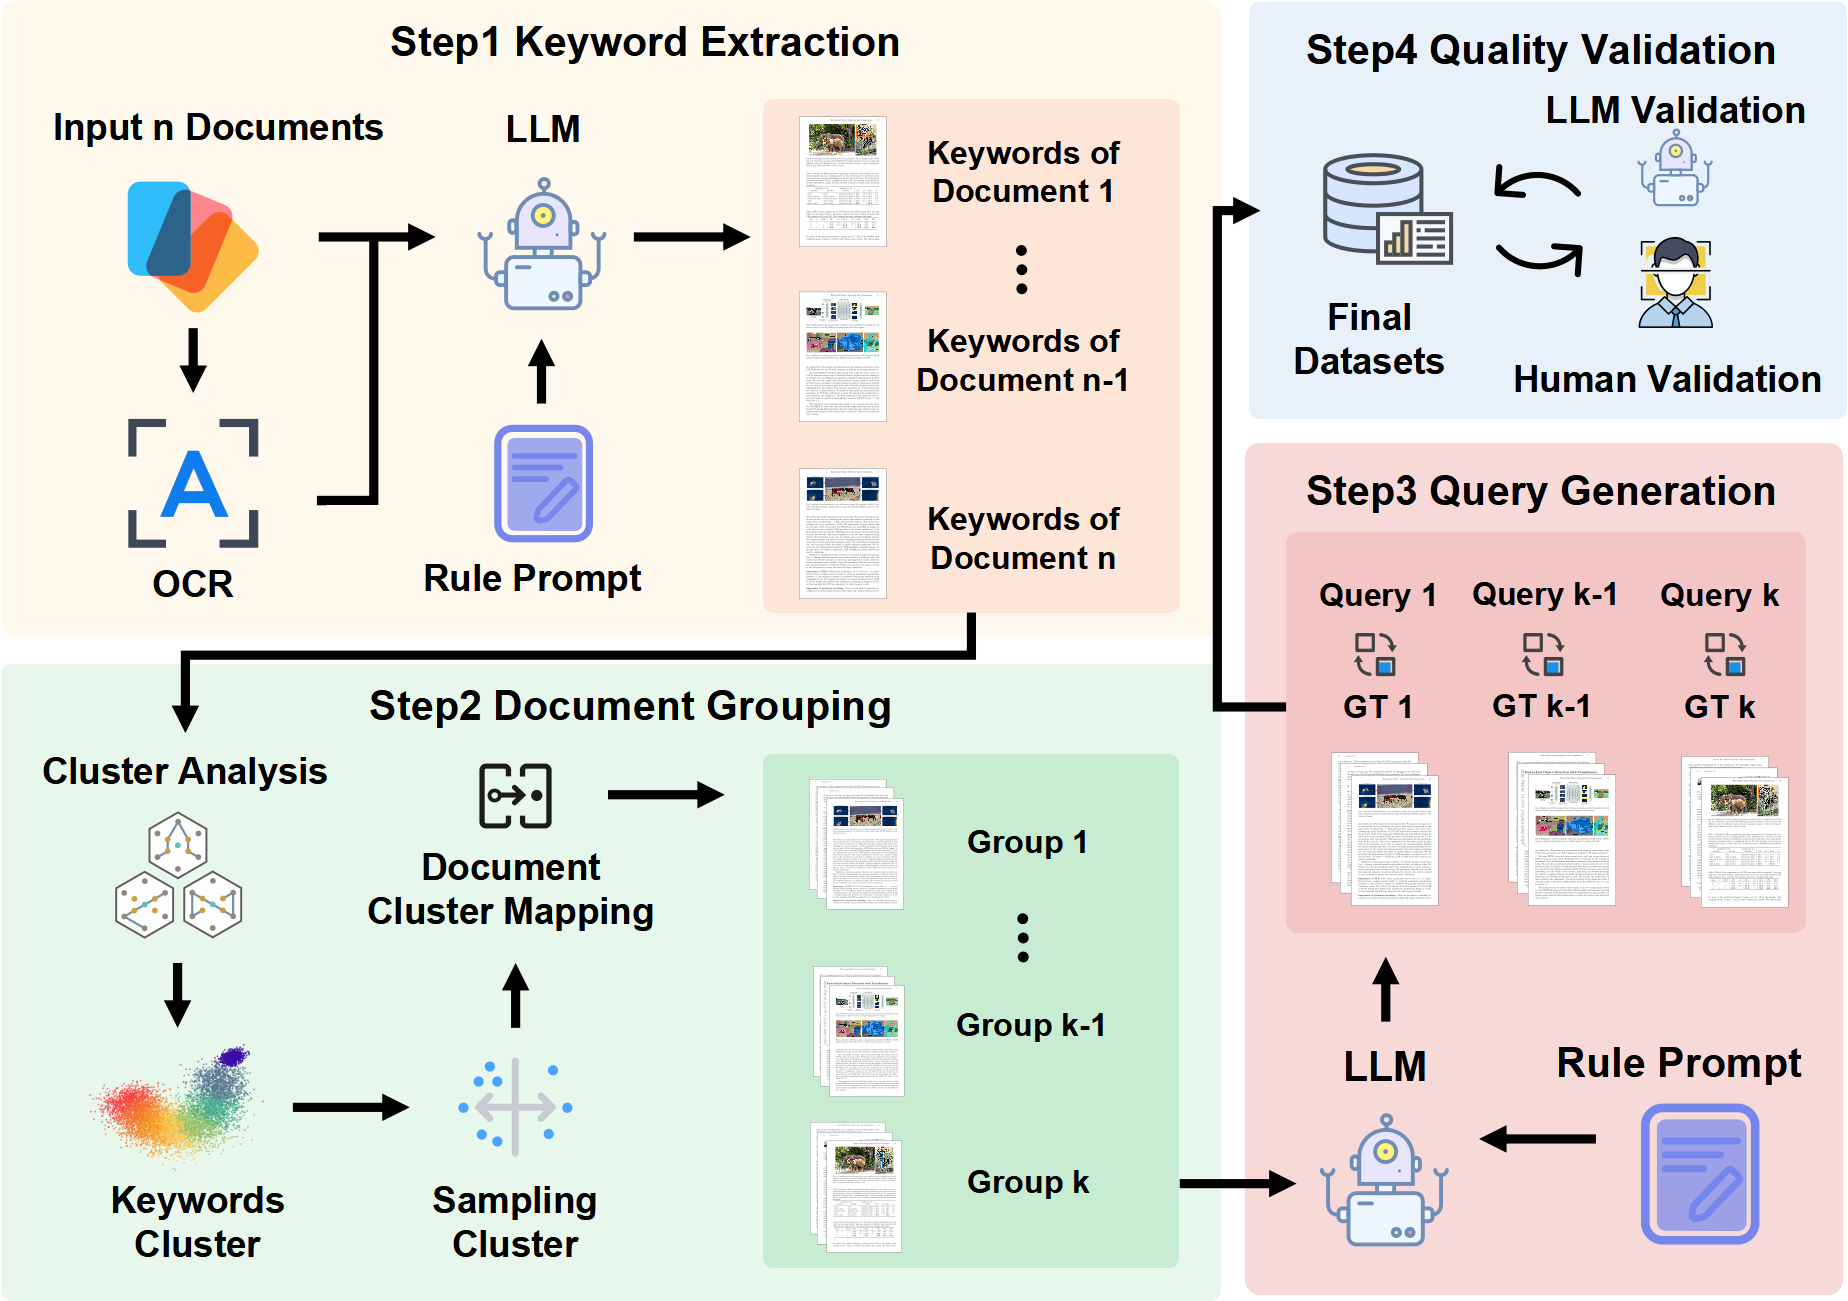
\includegraphics[width=\columnwidth]{figures/datasets_pipeline.png}
  \caption{Pipeline for constructing DocViRe. Documents are first processed with OCR and a large language model (LLM) to extract keywords. Cluster analysis then groups documents by topical similarity and assigns each to a group. For each group, an LLM generates document-level query-ground-truth pairs, which are validated by a second LLM pass and by human review to produce the final benchmark.}
  \label{fig:dataset-pipeline}
\end{figure}
\medskip

\begingroup
\setlength{\parskip}{0.4em}
\textbf{Keyword extraction.} For each input document, we first run OCR to obtain its text content. The OCR output, together with the raw document and a rule-based prompt, is then fed into a large language model. The LLM produces a structured set of keywords for the document, capturing its main topics and terminology at the \emph{document} level rather than isolated page fragments. These keyword sets summarize document-level themes and serve as the basis for grouping documents by topical similarity in the next step.

\textbf{Document grouping.} We perform cluster analysis over the extracted keywords to form a keyword-level clustering. After sampling and document-cluster mapping, each document is assigned to one of $k$ groups, so that documents within a group are topically similar (Group~1 through Group~$k$). This grouping creates document-level semantic neighborhoods and provides the basis for generating queries that may correspond to more than one relevant document.

\textbf{Query generation.} For each group, we use an LLM with a rule prompt to generate document-level query-ground-truth (GT) pairs. The prompt guides the model to produce natural retrieval queries that are answered by one or more complete documents in the group, describing the overall topic or higher-level information needs rather than specific sentences on a single page.

\textbf{Quality validation.} We apply a two-stage validation procedure to ensure benchmark quality. In the first stage, an LLM filters candidate query-document pairs that are only weakly related, such as those linked by superficial keyword overlap or a single-page local match. In the second stage, three human annotators exhaustively review all test-split samples and manually correct problematic queries and query-document pairs to ensure document-level relevance.

For query-document relevance, the three annotators labeled 98.8\%, 99.0\%, and 94.3\% of the checked pairs as relevant, respectively, with a three-way full agreement of 92.5\% and an at-least-two agreement of 98.8\%. For query validity, the three annotators marked 99.3\%, 99.7\%, and 100.0\% of all test queries as valid. On the test set, the three-way agreement reached 99.0\%. All invalid or inconsistent samples were subsequently corrected and re-annotated before finalizing the benchmark.

Importantly, human validation serves as the final quality-control step of the benchmark, rather than a lightweight spot check. All test-split samples are exhaustively reviewed by three annotators, and any invalid, ambiguous, or weakly document-grounded cases are manually corrected before inclusion. As a result, the final benchmark is determined by human-reviewed annotations, with LLM filtering used only as a preliminary screening step.

Additional statistics on split composition and positive-target distributions are provided in Appendix~\ref{sec:appendix-dataset}.
\endgroup